\documentclass[a5paper,12pt,twoside,openright]{scrbook}

\RequirePackage[utf8]{inputenc}
\RequirePackage[ngerman]{babel}
\RequirePackage{amsmath,amsthm,amssymb,amscd,color,graphicx}
\RequirePackage{environ}
\RequirePackage{framed}
\RequirePackage[protrusion=true,expansion=true]{microtype}
%\RequirePackage{lmodern}
\RequirePackage{multicol}
\RequirePackage{hyperref}

\usepackage[T1]{fontenc}
\usepackage{libertine}

\usepackage[onehalfspacing]{setspace}
\renewcommand*\theenumi{\alph{enumi}}
\renewcommand{\labelenumi}{\theenumi)}

\RequirePackage{minted}
\newminted{python}{}
\definecolor{light-gray}{gray}{0.91}
\newmintinline{python}{fontsize=\footnotesize,bgcolor=light-gray}
\newmintinline{text}{fontsize=\footnotesize,bgcolor=light-gray}
%\usemintedstyle{tango}

\newlength{\aufgabenskip}
\setlength{\aufgabenskip}{1.4em}
\newcounter{aufgabennummer}
\newenvironment{aufgabeUnshaded}[1]{
  \refstepcounter{aufgabennummer}
  \textbf{Aufgabe \theaufgabennummer.} \emph{#1} \par
}{\vspace{\aufgabenskip}}
\newcounter{lipnummer}
\newenvironment{lipUnshaded}[1]{
  \refstepcounter{lipnummer}
  \textbf{Lip \thelipnummer.} \emph{#1} \par
}{\vspace{\aufgabenskip}}
\NewEnviron{aufgabe}[1]{%
  \refstepcounter{aufgabennummer}%
  \begin{shaded}%
    \noindent\textbf{Aufgabe \theaufgabennummer.} \emph{#1} \par\medskip
    \noindent\BODY%
  \end{shaded}%
}
\NewEnviron{lip}[1]{%
  \refstepcounter{lipnummer}%
  \begin{shaded}%
    \noindent\textbf{Lip \thelipnummer.} \emph{#1} \par\medskip
    \noindent\BODY%
  \end{shaded}%
}
\newenvironment{aufgabeE}[1]{\begin{aufgabe}{#1}\begin{enumerate}}{\end{enumerate}\end{aufgabe}}
\newenvironment{LipE}[1]{\begin{lip}{#1}\begin{enumerate}}{\end{enumerate}\end{lip}}

\newenvironment{block}[1]{
  \begin{center}\textbf{#1}\end{center}
}{\vspace{\aufgabenskip}}

\definecolor{shadecolor}{rgb}{.93,.93,.93}

\title{Monty und Python werden Hacker \newline \small Ein Quellcode-Märchen}

\begin{document}

\maketitle
 
\tableofcontents 
 
\chapter{Wie das ganze begann oder: Wie benutze ich dieses Buch?} 

Liebe Leserin, lieber Leser.
Das folgende Buch dient dazu dir die Programmiersprache \emph{Python} nahezubringen.
Es gibt viele gute Bücher um Programmieren zu lernen, 
und insbesondere viele Bücher zu Python.
Ich persönlich lerne jedoch am liebsten mit viel Spa{\ss} und Fantasie.
Daher möchte ich dir gerne eine Geschichte erzählen und dir dabei ganz nebenbei 
Python beibringen, während du mitfieberst und die Abenteuer gemeinsam mit der Heldin erlebst.
Daher halten wir uns nun gar nicht lange auf und beginnen mit unserer Geschichte...


\begin{center}
 
\includegraphics[scale = 0.1]{monty1.png}
\end{center}
Es war einmal ein Mädchen namens Monty mit sehr schwarzen Haaren und einem sehr roten Mantel.
Monty war ein Mädchen wie so viele andere auf der Welt, so mochte sie beispielsweise Rosenkohl 
gar nicht und a{\ss} ihn nur den Eltern zuliebe unter Einsatz ihres ganzen Mutes.
Sie liebte Regenwürmer - eigentlich liebte sie alles was mit \glqq Regen-\grqq begann - und in der Schule kümmerte sie sich gerne 
um die Schnecken im Aquarium. 
Aber was Monty ganz besonders liebte, war Mathematik und Logik.
Auch war sie schon immer fasziniert von Computern gewesen (interessante Geräte, fiepen und blinken 
und können dir aber die Wegbeschreibung zu Tante Hilda liefern!).
Monty hätte nun ein seeliges, ruhiges Leben haben können, mit viel Schnecken und Logik, 
aber eines Tages änderte sich das ganz plötzlich.
Als Monty eines Tages bei Regen den Garten betrat um Regenwürmer vor dem Ertrinken zu retten, 
tauchte plötzlich eine fliegende Untertasse vor ihr auf. 
Auf den zweiten Blick stellte, sie fest, dass es sogar eine Tasse mitsamt Untertasse war.
Heraus schlüpften blaue und rosa Quallen --so sahen sie zumindest aus-- und schnurstracks hatten sie Monty entführt.


\begin{center}
 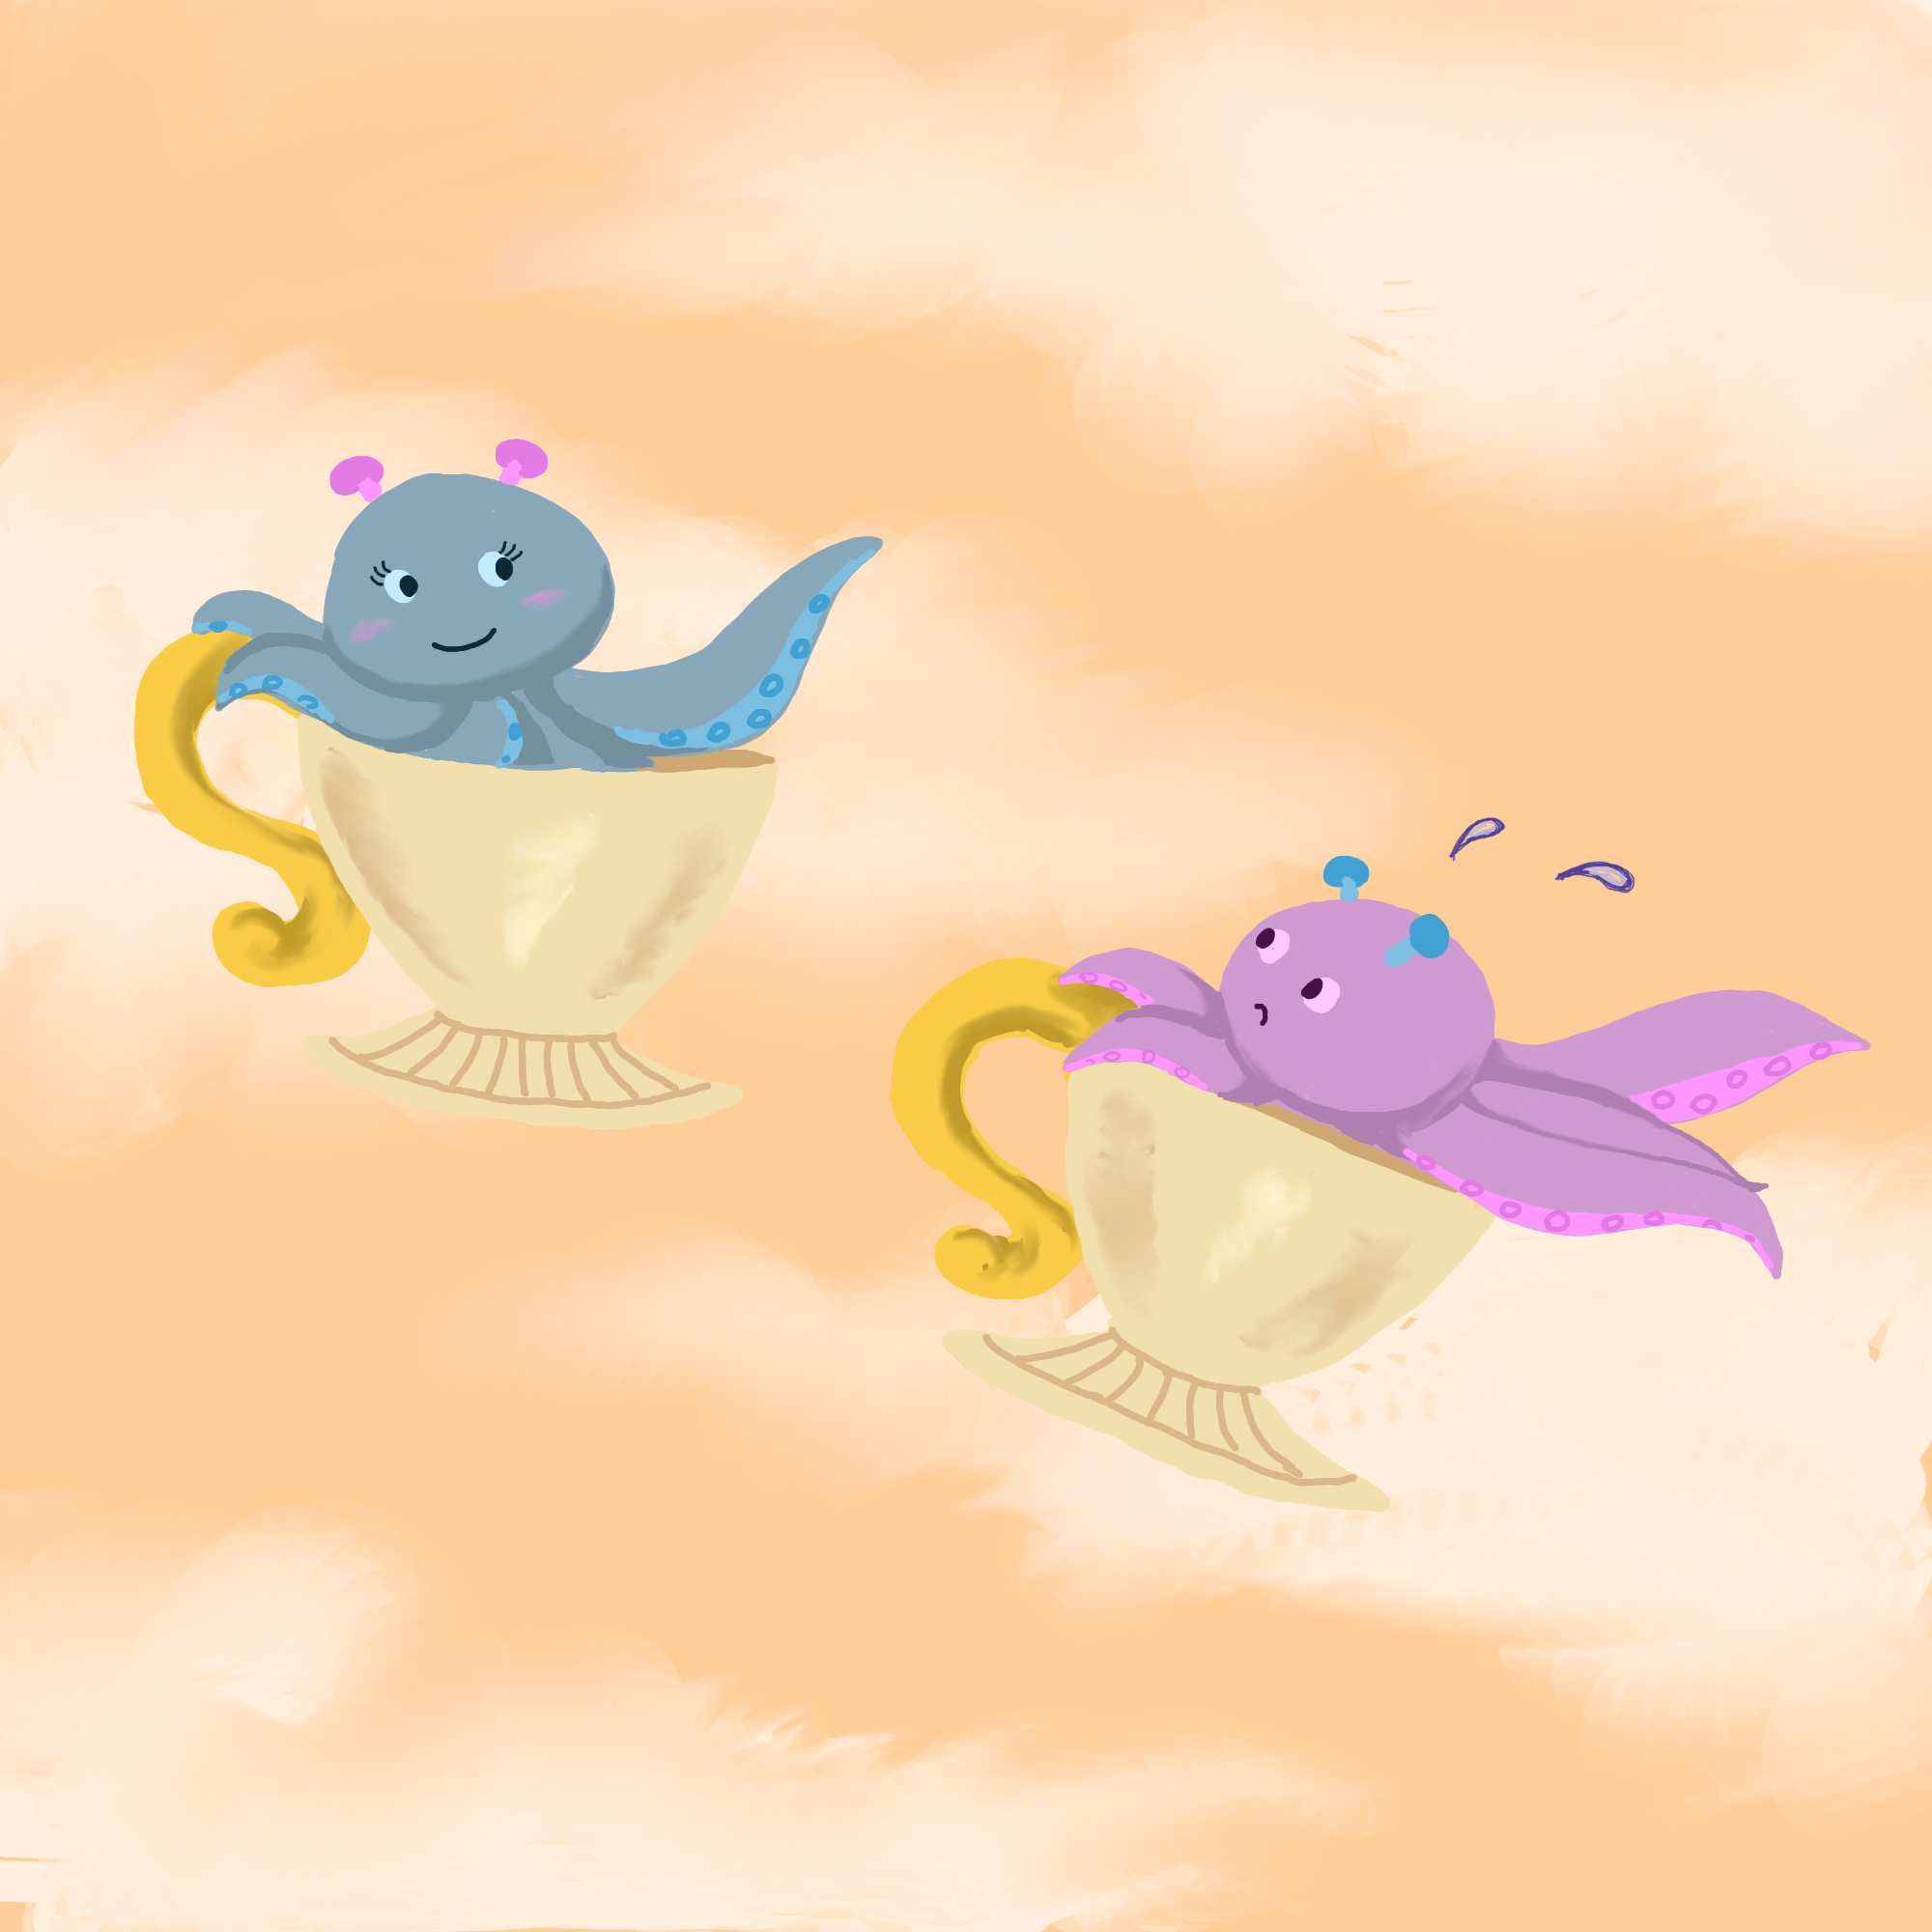
\includegraphics[scale = 0.1]{aliens.png}
\end{center}
Monty hätte zu gerne den Grund dafür erfahren, aber leider verstanden die Quallen ihre Sprache nicht und umgekehrt.
Nach einem langen Teetassenflug mit einigen Turbulenzen landeten sie in einem dichten Dschungel und dort traute Monty ihren Augen nicht mehr.
Dort parkte eine gigantische Teekanne, wohl das Mutterschiff wie Monty folgerte, und viel, viel mehr quallenartige Aliens schwirrten umher.

Plötzlich kam ein Ringelstrumpf auf Monty zu.
"`Guten Tag, ich bin die Python \emph{Python}, aber die meisten nennen mich \emph{Py}."' wurde Monty begrüsst.

"`Aber du bist doch ein Strumpf!"' entgegenete Monty verdattert.

Py sah sie böse an. 
"`Natürlich nicht, ich bin eine waschechte gefährliche Python. Und ich wurde von denen hier entführt, genau wie du.
Ich verstehe nämlich ihre Sprache und soll für dich übersetzen."'


\begin{center}
 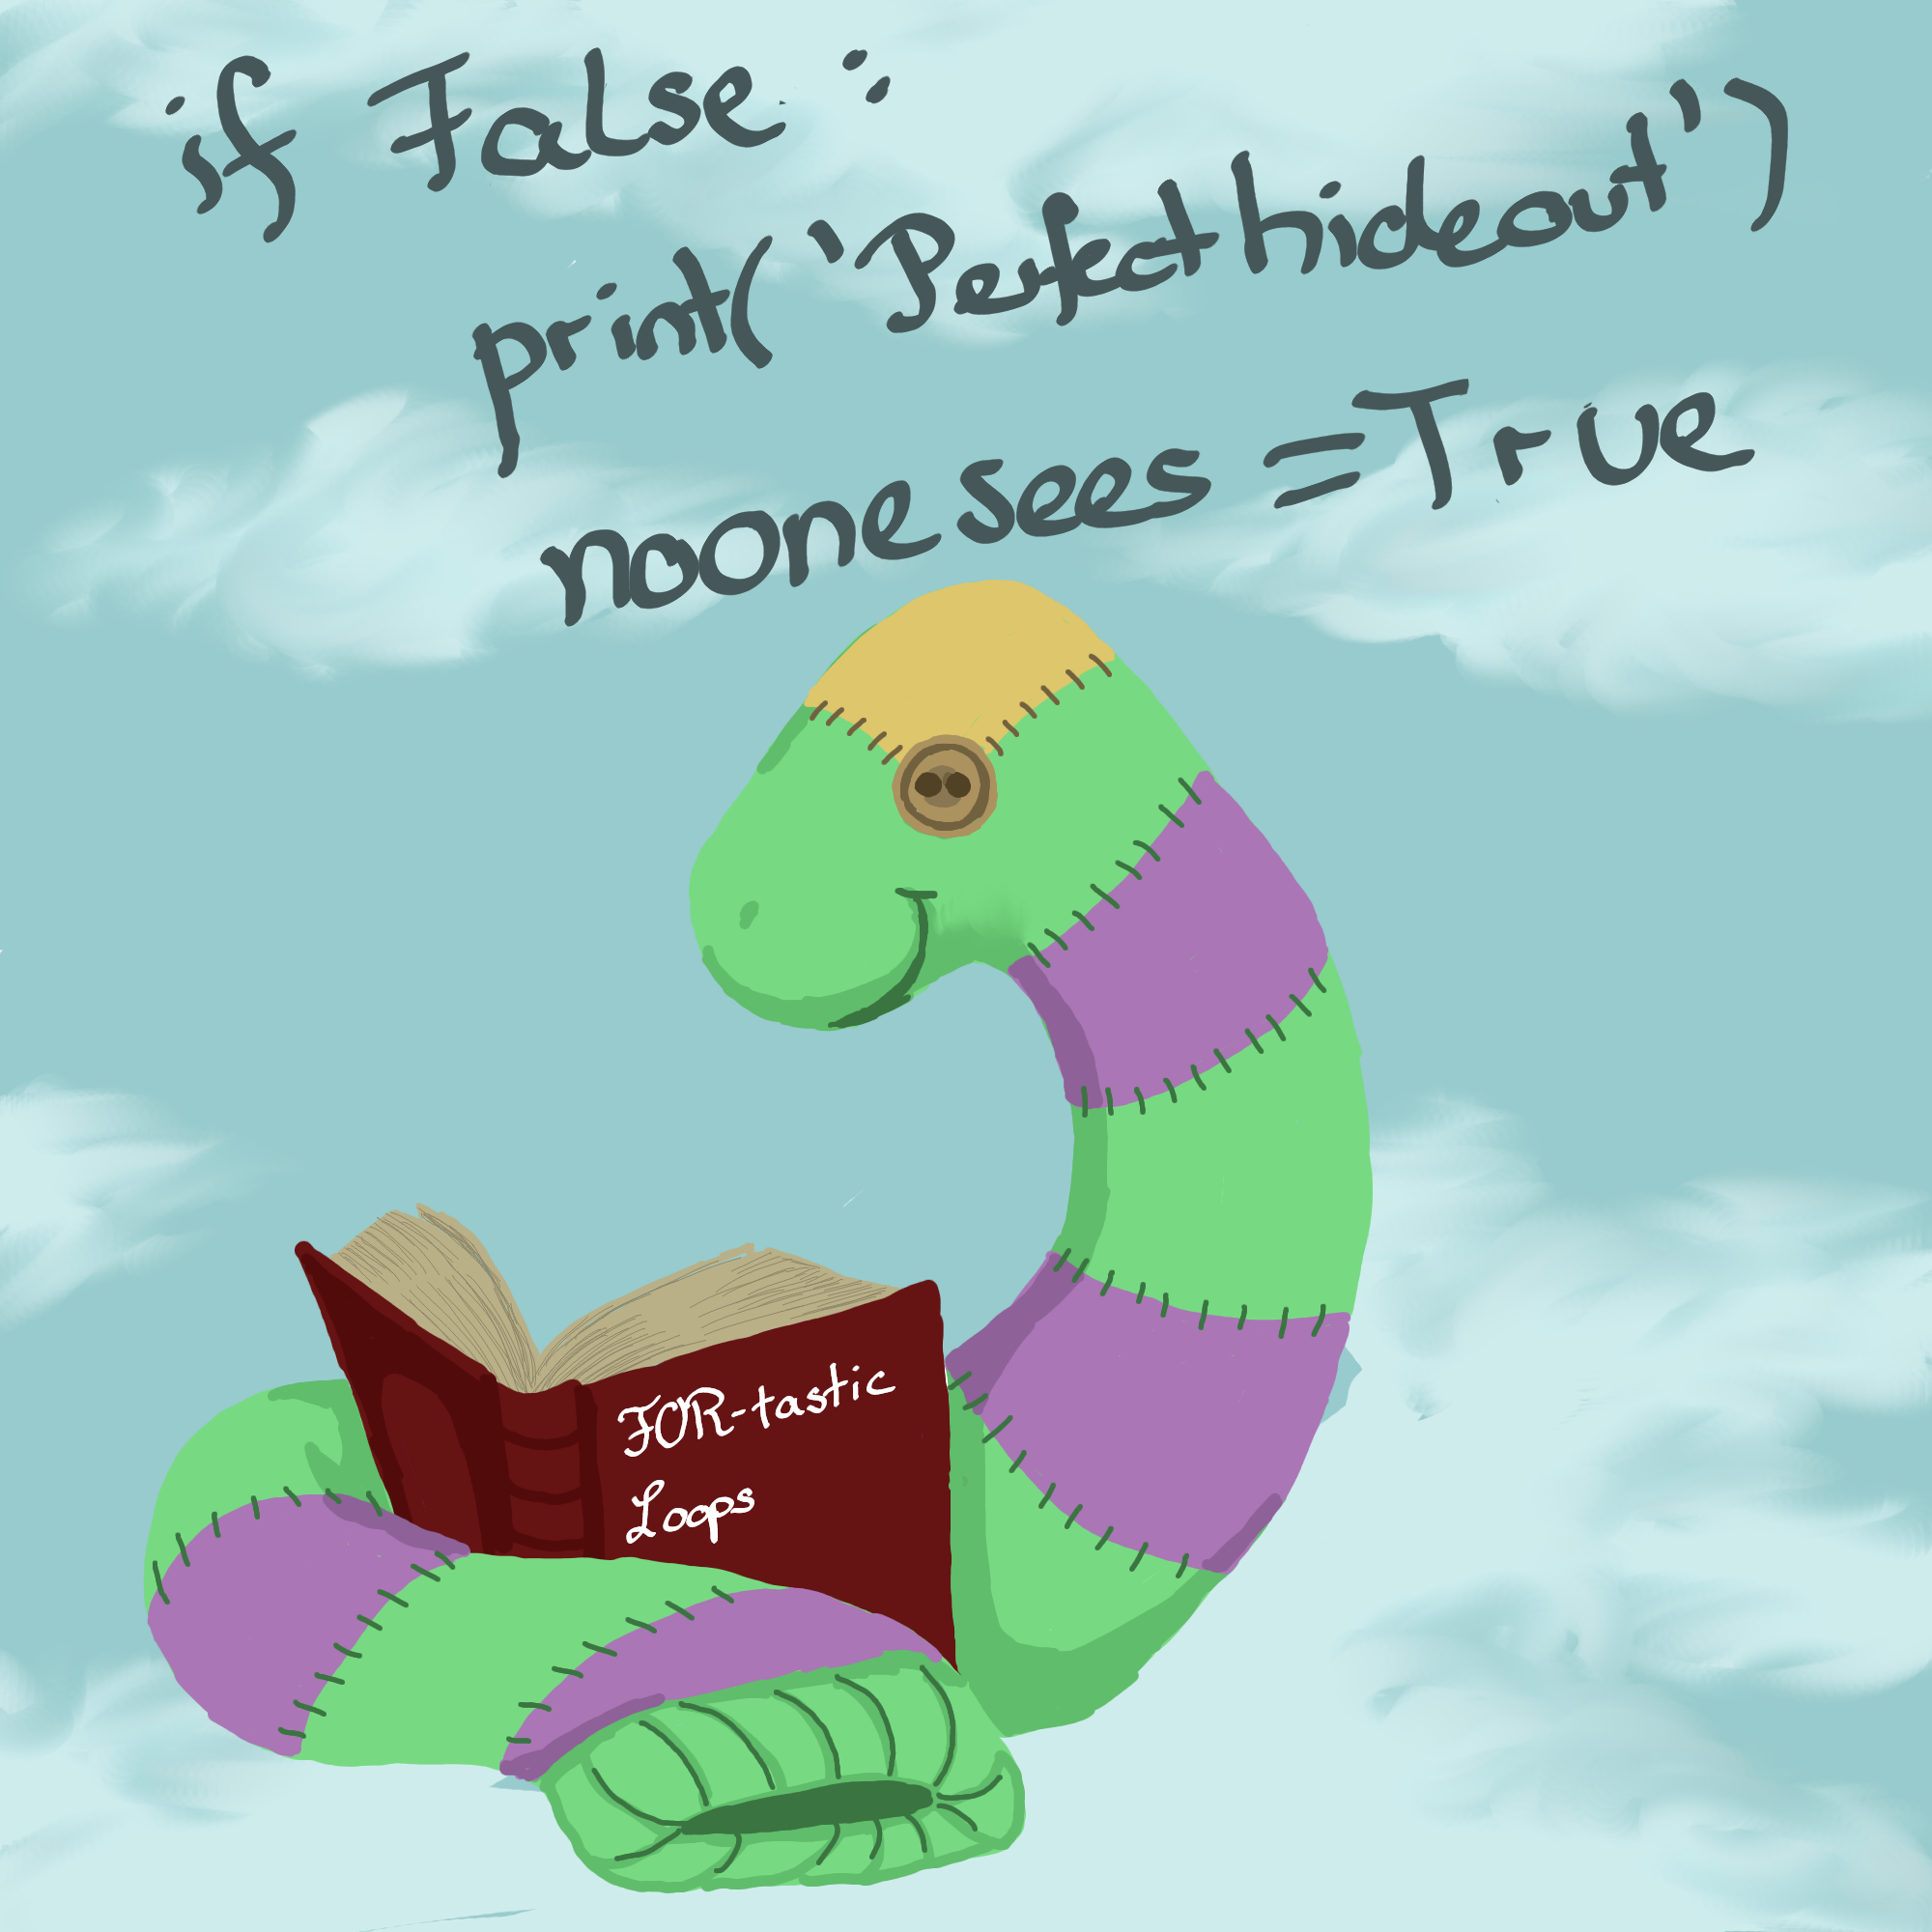
\includegraphics[scale = 0.1]{py.png}
\end{center}
"`Aber was wollen sie denn überhaupt von mir?"' fragte Monty verwirrt.

-"`Ihr Raumschiff ist beschädigt und sie brauchen jemanden zur Reperatur. Dazu müssen wir in ihrer 
sonderbaren Programmiersprache programmieren und sie glauben, du bist perfekt dafür!"'

"`Ich weiß nicht wie man programmiert!"' entgegnete Monty verwirrt.

"`Das lernst du mit mir zusammen. Du magst doch Mathematik und Logik, oder? Dann bist du genau die Richtige, versprochen!"'

Monty fragte sich, ob sie das schaffen würde. Aber die Quallen sahen so traurig und heimatlos aus, dass sie ihnen helfen wollte.
Au{\ss}erdem wollte sie auch wieder nach Hause zurück. 

"`Keine Angst, wenn wir fertig sind, bringen sie uns wieder zurück!"' erklärte Py in diesem Moment, 
als hätte sie Montys Gedanken lesen können.

-"`Also gut Py. Ich mache es."'
 
\chapter{Variablen}

"`Wie können wir nun das Raumschiff der Aliens wieder in Gang bringen?"' wollte Monty wissen.

Py deutete auf drei Aliens, die direkt auf sie zukamen und eine Truhe mit sich schleppten.

"`Ich vermute, wir sollen sie öffnen, Monty."' 

Das taten sie denn auch und zunächst fanden sie in der Kiste nichts au{\ss}er einigen beschriebenen Pergamentblättern und einem kleinen Computer.

"`Ich glaube, wir müssen zuerst den Hauptcomputer aufwecken, Monty. Und hier steht beschrieben wie."'
Py besah die Pergamente und Monty war sehr froh, dass Py die Sprache und Schrift der Aliens verstand.

"`Gut, dann fangen wir doch gleich mit der ersten Lektion an!"' rief Monty aufgeregt.

-"`Zuerst müssen wir das Konzept von \emph{Variablen} verstehen."'  

"`Variablen?"'

Py deutete auf den Computer, den sie zum Programmieren bekommen hatten.
"`Starte mal den Computer und öffne die \emph{Konsole}! Die Konsole ist ein kleines schwarzes Fenster, du findest es bei deinen Programmen.
 Manchmal wird sie auch \emph{Terminal} oder \emph{Shell} genannt. Dann gibst du \emph{python} ein und drückst \emph{Enter}."'

Monty gehorchte und blickte auf den schwarzen Bildschirm - die Konsole, wie Py ihn genannt hatte.

"`Sehr gut. Zunächst musst du wissen, dass diese Programmiersprache ein besserer Taschenrechner ist. 
Tipp doch bitte mal 2 + 3 in die Konsole ein, Monty."'

So tat Monty denn auch.
"`Merkwürdig. Es passiert nichts?"' wunderte sie sich.

"`Ja natürlich nicht. Du musst ja auch noch die \emph{Enter}-Taste drücken."' dirigierte Py.

Jetzt erschien eine 5 auf dem Bildschirm.

"`Wow, super!"' rief Monty. "`Kann ich damit alles ausrechnen?"'

"`Versuchs doch mal."' entgegnete Py.

\begin{aufgabe}{Einfache Rechenoperationen}
Führe folgende Rechnungen in der Konsole aus:
\begin{itemize}
 \item[a)] 3 + 4
 \item[b)] 2 * 3
 \item[c)] 5 - 2
 \item[d)] 8 / 2 
\end{itemize}
\end{aufgabe}

"`Das Problem ist nur, dass das Programm sofort wieder vergisst was man gerechnet hat."'
meinte Py.

-"`Wie meinst du das?"'

"`Nun sieh mal, ich hatte die Rechnung 2 + 3 und habe als Ergebnis die 5 bekommen. Eventuell möchte ich jetzt mit der 5 weiterrechnen, 
aber dazu müsste ich sie neu eintippen. Sie ist nirgends \emph{gespeichert}."' erklärte Py.

-"`Kann man sie denn speichern?"'

"`Ja und dazu sind die Variablen da. Eine Variable musst du dir vorstellen wie eine Geschenkbox. 
Du kannst sie aufmachen und etwas hineingeben oder herausnehmen. Wenn du einen Wert speichern willst, musst du 
ihn in eine solche Box geben, der du einen Namen gibst. Dann kannst du sie - so lange du das Programm nicht beendest - 
jederzeit öffnen und hineinsehen, was sich darin befindet."'

-"`Eine Box also. Und wie mache ich die?"'

"`Das steht auch hier. Gib mal folgendes in die Konsole ein: \textit{abc = 5} und drücke enter."'

"`Jetzt ist gar nichts passiert?"' fragte Monty.

-"`Ja so scheint es. In Wahrheit hast du jetzt aber eine Box erzeugt, die den Namen \textit{abc} trägt. 
Und darin befindet sich nun der Wert 5. Gib mal abc ein und drücke enter."'

"`Tatsache, er zeigt mir die 5 an!"' freute sich Monty.

"`Du kannst mit diesen Boxen auch rechnen."' erklärte Py.

Jetzt musste Monty lachen.
"`Wie soll ich denn mit Boxen rechnen? Rechnen kann man doch nur mit Zahlen!"'

"`Na, überlege doch mal, Monty. In den Boxen haben wir ja Zahlen!"'
Py deutete auf den Bildschirm. 

"`Gib doch mal folgende Dinge ein: a = 5,enter, b = 7, enter.
z = a + b."'

Monty tat wie geheißen.

"`Was ist nun z, was meinst du, Monty?"'

Monty sah auf den Bildschirm.
"`Da du meintest, dass mit dem Boxeninhalt gerechnet wird und in a die Zahl 5 steckt, sowie in b die Zahl 7, vermute ich dass 5+7 = 12 herauskommt."'

Py grinste sie an.
"`Probiers aus, gib z ein und drücke enter."'

"`Ha, super, ich habe es gewusst."' freute sich Monty.

\begin{aufgabe}{Variablenspiele}
 Meistere folgende Aufgaben:
 \begin{itemize}
  \item[a)] Erstelle die Variable p und weise ihr den Wert 3 zu.
  \item[b)] Erstelle die Variable q und weise ihr den Wert 12 zu.
  \item[c)] Berechne q/p und speichere das Ergebnis in der Variable r.
  \item[d)] Gib die Inhalte aller Variablen aus.
 \end{itemize}
\end{aufgabe}

In diesem Moment wurden die kleinen Aliens v\"ollig aufgeregt und deuteten begeistert auf
einen Computer, den Py zuvor als Hauptcomputer bezeichnet hatte.
Er war etwa so groß wie Monty, wenn man den Bildschirm mitz\"ahlte, der 
wir ein Kopf auf ihm thronte.
Der Korpus des Computers war seltsam kugelförmig und hatte viele Tasten und Kn\"opfe 
und vorne befand sich eine Tastatur, als ruhe sie auf seinem kugeligen Bauch.

Einer der Aliens dr\"uckte einen großen, runden Knopf, 
woraufhin dieser in allen Farben des Regenbogens zu leuchten begann.
Auf dem schwarzen Monitor erschien einiger Code.
Py besah sich das Ganze um sich einen Reim auf die Problemstellung zu machen.

"`So, Monty, es scheint mir hier folgendes Problem im Wege zu stehen. 
Siehst du die Variablen \textit{frosch} und \textit{ente} in diesem Code?"'

Monty nickte und wunderte sich \"uber die Variablennamen.

"`Tja, da siehst du warum man Variablen gute Namen geben sollte, am besten Namen die ihre Funktion beschreiben. 
Eine Variable, die eine Kreisfl\"ache enth\"alt w\"urde ich ja nun \textit{kreisflaeche} oder \"ahnlich nennen, aber sicher nicht Ente."'

Monty kicherte.

"`Du musst das Ernst nehmen. Durch diese sonderbaren Namen haben die Aliens n\"amlich versehentlich die Inhalte der Variablen 
\textit{Frosch} und \textit{Ente} vertauscht. 
Um das Ganze hier also zu reparieren, musst du die Inhalte hier an dieser Stelle wieder zur\"ucktauschen!"'

\begin{aufgabe}{Die erste Pr\"ufung}
 Erstelle dir ebenfalls zwei Variablen \textit{Frosch} und \textit{Ente} und weise ihnen 
 verschiedene Werte zu, die du aussuchen kannst.
 Vertausche jetzt die Inhalte der beiden Variablen. Kannst du das?
\end{aufgabe}

F\"ur dieses R\"atsel musste Monty eine ganze Weile \"uberlegen und du vielleicht auch.
Auf der n\"achsten Seite erf\"ahrst du wie es weiter ging. (XXX)

Schlie{\ss}lich kam Monty auf eine Idee.
"`Also direkt kann ich es nicht machen, Py. Wenn ich \textit{Ente} = \textit{Frosch} schreibe, ist n\"amlich der Inhalt von \textit{Ente} weg 
und umgekehrt. Also mache ich mir eine neue Variable!"'

Monty tippte:
\begin{pythoncode*}{escapeinside=||}
hilfe  = ente
ente   = frosch 
frosch = hilfe
\end{pythoncode*}
%\textit{Hilfe} = \textit{Ente}
%\textit{Ente} = \textit{Frosch}
%\textit{Frosch} = \textit{Hilfe}

und Py ließ das Programm laufen.
Da kam Leben in den kleinen Computer, er fing an zu rattern und zu pfeifen 
wie ein alter Wasserkessel und schließlich erschienen auf dem Bildschirm zwei gro{\ss}e Augen.

"`Guten Tag."' sagte eine mechanische Stimme aus dem kugeligen Korpus.

"`Ich bin der Hauptcomputer LinWinMackenzie Vierkern von Dampfstrahl, kurz Linnie."'

"` \"Ahm, Guten Tag."' erwiderten beide verwirrt den Gru{\ss}, 
hatten sie doch noch nie einen so h\"oflichen Computer kennen gelernt.

"`Vielen Dank, dass ihr mich aufgeweckt habt. Ab jetzt kann ich euch mit Rat und Tat zur Seite stehen."'
erkl\"arte Linnie.
"`Soll ich euch probeweise einen geben?"'

Monty nickte. "`Ja, nur zu, was wei{\ss}t du, was wir nicht wissen?"'

-"`Es war sehr schlau, wie ihr mich aufgeweckt habt. 
Aber es gibt in dieser Sprache noch eine andere M\"oglichkeit Variableninhalte zu tauschen."'

Und da erschien auf dem Bildschirm
\begin{pythoncode}
 a,b = b,a
\end{pythoncode}
%\textit{a, b} = \textit{b, a}



\begin{aufgabe}{Der kurze Tausch}
 Erstelle zwei Variablen \textit{a,b} und weise ihnen verschiedene Inhalte zu, 
die du wieder frei aussuchen kannst.
 Probiere den Vorschlag von Linnie aus.
\end{aufgabe}

Da staunten Monty und Py nicht schlecht und f\"uhlten sich 
beruhigt und ermuntert, denn mit einer klugen Hilfe wie Linnie 
w\"urden sich zuk\"unftige Pr\"ufungen leichter l\"osen lassen.

\begin{aufgabe}{Linnips}
 Liebe Leserin, lieber Leser,

 ab sofort ist Linnie dabei. 
 Wenn am Seitenrand dieses Symbol auftaucht,
 gibt Linnie dir einen Tipp, den du lesen kannst, aber nicht musst. 
 Da die Tipps alle von Linnie stammen, nennt er sie Lips.
\end{aufgabe}

\chapter{Schleifen}

%Steuermodul reparieren
%n Eck
%erwischt werden? Urwald 

Nachdem Monty und Py nun Linnie restauriert hatten, war an eine Pause natürlich nicht zu denken.

"`Wie genau sollen wir nun vorgehen, Linnie?"' erkundigte sich Monty.

"`Ihr seid informiert worden, dass das Mutterschiff beschädigt worden ist? 
Nun, eines der größten Probleme ist wohl das ausgefallene Steuermodul.
Selbst wenn weiter nichts defekt wäre, könnte man dieses Schiff nicht bewegen.
Wir müssen uns also um das Steuermodul kümmern!"' erklärte Linnie.

Py und Monty sahen sich an und zuckten beide mit den Schultern.

"`Also, von Werkzeug habe ich wirklich keine Ahnung."' erklärte Py verdrossen.

"`Nein, meine Lieben, wir müssen natürlich ein Programm schreiben."' beruhigte Linnie die beiden.
"`Das Problem ist nur, dass das diesmal ein bisschen schwieriger wird. 
Daher muss ich euch erstmal mit dem Konzept von \emph{Schleifen} vertraut machen, sofern ihr das noch nicht kennt."'

Monty blickte verstohlen auf ihre Schuhe. Vermutlich waren solche Schleifen nicht gemeint.
Daher schüttelten Monty und Py zeitgleich den Kopf, wobei Pys Zunge ulkig mitwackelte.

"`Okay, lasst uns anfangen! Öffne doch mal wieder die Konsole, Monty!"' bat Linnie.

Monty gehorchte und wartete auf weitere Arbeitsanweisungen. 

"`So, Monty, gib mal bitte \emph{print("Hallo")} ein und drücke Enter."' 
 
"`Aha, er schreibt mir \emph{Hallo} auf den Bildschirm!"' fasste Monty die Geschehnisse zusammen.

-"`Ganz genau! Das \emph{print} bedeutet soviel wie, nun ja \ldots{} drucken. Also im Prinzip: Drucke das Wort Hallo auf den Bildschirm, in unserem Fall.
Mach dir doch mal eine Variable a, weise ihr irgendeinen Wert zu und probiere print(a) aus!"'
 
\begin{aufgabe}{Wir können drucken}
 Führe die von Linnie gestellte Aufgabe aus. Was fällt dir auf?
\end{aufgabe}

"`Mit print kannst du jetzt ab sofort alles ausgeben."' erklärte Linnie.

"`Das ist ja schön und gut, aber was hat das mit Schleifen zu tun?"' fragte Monty in die Runde.

-"` Dazu kommen wir jetzt. Stell dir mal vor, jemand möchte die Variable a nicht einmal auf dem Bildschirm ausgeben, sondern 7 mal."'

"` Das ist ja nun kein Hexenwerk."' meinte Monty. "` Dazu muss ich doch nur sieben mal print(a) schreiben und dann haben wir das Gewünschte."'

"`Das ist zweifelsohne wahr."' bestätigte Linnie. "`Aber was ist, wenn man es 100 mal ausgeben will? 
Irgendwann wird es doch wirklich lästig, so oft den gleichen Befehl zu tippen, nicht wahr?"'

"`Linnie, wozu sollte ich das denn auch wollen? Das ergibt doch keinen Sinn."' lachte Monty.

"`Nehmen wir doch einmal an, du sollst das machen. Dann verrrate ich dir jetzt wie -- und zwar ohne, dass du hundert mal dasselbe tippen musst.
Das ganze macht man mit einer Schleife!"'

"`Na, dann erklär mal!"' riefen Monty und Py im Chor.

-"` Bitte tippe mal ein \emph{for i in range(100):} . Dann drückst du enter. 
Jetzt wird es sehr wichtig. Rücke bitte die nächste Zeile mit der \emph{Tabulatortaste} um eins ein. Das ist die Taste auf der gleich zwei lange Pfeile sind, die 
in entgegengesetzte Richtung schauen. Hast du das? Sehr gut! 
Jetzt tippst du \emph{print(a)} und enter. Tadaa!"'

XXX links neben dem Q?

\begin{aufgabe}{Deine erste Schleife}
 Probiere das gleich mal aus. 
 Teste zudem folgendes: Rücke das print(a) nicht ein. Was passiert?
\end{aufgabe}

"`Wahnsinn, alles ist voll mit meiner drei!"' rief Monty (denn das war der Wert, den Monty der Variable a zugewiesen hatte. 
Welchen hattest du gewählt?)

"`Ich erkläre euch jetzt, was wir da gemacht haben. Wir haben eine sogenannte \emph{for}-Schleife geschrieben.
Dieses Kommando oben bedeutet, dass der Inhalt der Schleife 100 Mal durchlaufen wird -- das ist die Zahl in dem Befehl \emph{range}.
Zu der Schleife gehört jeglicher Code der eingerückt wird. Hätten wir das print nicht eingerückt, hätten wir praktisch eine Schleife geschrieben, 
die \emph{leer} ist, es wäre nichts geschehen, und danach wäre a einmal gedruckt worden.
Aber alles eingerückte nach dem for wird 100 mal ausgeführt. Hier war das das Drucken.
Und die for-Schleife hat noch eine Spezialität. In dem obigen Befehl gibt es nämlich noch die Variable i.
Die durchläuft nacheinander alle Zahlen von 0 bis 99, also 100 Stück."'

"`Warum nicht von 1 bis 100?"' fragte Monty irritiert.

"`Och, das liegt einfach daran, dass unsere kleinen Aliens hier die 0 so sehr lieben, dass sie immer bei der 0 anfangen zu zählen."' grinste Linnie.

\begin{aufgabeUnshaded}
{Fortastisch}
 Probiere mal die folgenden Schleifen aus! Achte dabei gut auf die Einrückung.
 Die Variable a solltest du ja zuvor bereits erstellt haben.
 Was passiert, wenn man die Einrückung missachtet oder ändert?
%  \begin{pythoncode}
%   a
%  \end{pythoncode}
 \begin{itemize}
  \item \begin{pythoncode}
         for i in range(11):
	     print(i)
        \end{pythoncode}
%for i in range(11): print i
  \item \begin{pythoncode} 
         for i in range(5):
             a = i
             print(a)
        \end{pythoncode}
% \begin{verbatim}a= 0
%for i in range(5):
%print(i)%\end{verbatim}
  \item \begin{pythoncode}
         for i in range(7):
             a = a + i
        \end{pythoncode}
  %for i in range(7): a = a + i
 \end{itemize}
\end{aufgabeUnshaded}
 
 %for schleife schreiben lassen, zB alle Zahlen aufaddieren? sowas hätte ich gern drin.
 
 \begin{lip}{}
  Im ersten Beispiel wird bei fehlender Einrückung eine Fehlermeldung erscheinen.
  Die Variable i existiert nämlich nur im Rahmen der for-Schleife. 
  
  Im zweiten Beispiel wird a in jedem Schritt der aktuelle Wert von i zugewiesen. Rückt man beides nicht ein, kommt wieder die Fehlermeldung.
  Ob print eingerückt ist, entscheidet darüber ob in jedem Schritt der Schleife a ausgegeben wird oder nur am Ende.
 \end{lip}

"`So, jetzt kommen wir unserem Problem schon näher. Monty, mach doch mal bitte einen Internetbrowser auf 
und gib die Adresse www.elfenteich.de/ppp ein."'

Monty folgte der Anweisung nicht ohne sich wieder einmal zu wundern.

"`Jetzt sehe ich ein weißes Feld vor mir. Soll ich dort etwas tippen? "'
fragte Monty. 

Linnie räusperte sich kurz und Py und Monty waren überaus fasziniert davon, dass ein kleiner Computer 
die Wirkung von bedeutungsvollem Schweigen kannte.

"`Jetzt wird es wirklich wichtig. Wir wollen ja das Raumschiff wieder in Gang bringen. 
Insbesondere soll es herumfahren können. Gebt bitte den Befehl \emph{forward(100)} ein und führe das Programm aus."'

\begin{aufgabeUnshaded}{Wir beginnen zu laufen}
 Besuche ebenfalls die Website.
 Gib in dem weißen Feld nacheinander die Befehle
 \begin{pythoncode}
  forward(100)
  left(90)
  forward(100)
 \end{pythoncode}
 %forward(100), left(90), forward(100) 
 ein und führe das Programm aus.
 Was stellst du fest?
\end{aufgabeUnshaded}

Nun passierten zwei Dinge gleichzeitig und beide kamen sehr überraschend.
Auf dem Bildschirm erschien ein schwarzer Pfeil und gleichzeitig bewegte sich das Raumschiff um etwa einen Meter.
Monty und Py mussten sich aneinander klammern um nicht umzufallen, so sehr ratterte das Raumschiff und wackelte.
Bereits kurz darauf umarmten sie sich und lachten von Herzen - 
sie hatten es geschafft, das Raumschiff bewegte sich!

Linnie wartete taktvoll, bis beide sich wieder beruhigt hatten. 
Dann erklärte er die Steuerungsbefehle.
Der Befehl \emph{forward(100)} bewegt das Raumschiff um 100 cm, also einen Meter 
in die Richtung, in die es blickt.
Der Befehl \emph{left(90)}, bzw. \emph{right(90)} dreht das Raumschiff um 90 Grad nach links, bzw, nach rechts ohne es zu bewegen.
Der Winkel kann jedoch variiert werden, so entspricht \emph{right(45)} beispielsweise einer Rechtsdrehung um 45 Grad.

\begin{aufgabe}{Steuerungsspiele}
 Lass dein Raumschiff erstmal beliebig laufen (Zickzack, im Viereck, ...), indem du die obigen Befehle aneinander hängst 
 und ausprobierst.
\end{aufgabe}

\begin{aufgabe}{Das Haus des Nikolaus}
 Schaffst du es, das Raumschiff so zu steuern, dass das Haus des Nikolaus in einem Zug 
 abgelaufen wird? 
\end{aufgabe}

 \begin{lip}{}
 Für das Haus des Nikolaus wirst du mit dem Winkel bei left und right sowie mit den Längen experimentieren müssen.
 \end{lip}

Nachdem Monty und Py ihren Spa{\ss} damit hatten, das Raumschiff umherwandern zu lassen, ergriff Linnie erneut das Wort. 

"`Selbstverständlich kannst du hier auch Schleifen benutzen um mehrere Strecken auf einmal zu gehen.
  Probiere das doch mal aus. Lass das Raumschiff in einem Viereck laufen und wiederhole das dreimal."'
  
Monty tippte folgendes ein:  
%\begin{verbatim}
\begin{pythoncode}
for i in range(3):
   forward(100) 
   right(90)
   forward(100)
   right(90)
   forard(100)
   right(90)
   forward(100)
\end{pythoncode}

%\end{verbatim}

\begin{lip}{}
 Der Code in der Schleife zeichnet ein Rechteck. 
 
 Teste diesen Code zuerst alleine und danach den gesamten Code von Monty.
\end{lip}


``Du kannst den Code übrigens noch deutlich vereinfachen.'' erklärte Linnie.

``Wie denn?'' wunderten sich Monty und Py.

``Du hast ja gesehen, dass es vorgefertigte Befehle gibt. forward(100) beispielsweise.
Wir können uns jetzt eigene Befehle bauen. Tippe mal folgendes:''

\begin{aufgabeUnshaded}{Eigene Befehle erfinden}
 Führe Linnies Code aus. Gib folgendes ein:
\begin{pythoncode}
def viereck(n):
    forward(n) 
    right(90)
    forward(n)
    right(90)
    forard(n)
    right(90)
    forward(n) 
    
for i in range(3):
    viereck(100)  
\end{pythoncode}
\end{aufgabeUnshaded}

``Aha, die Variable n steht also für die Seitenlänge des Vierecks.'' folgerte Monty.
``Denn wenn ich viereck(100) ausführe, fahren wir jeweils 100 cm in jede Richtung, 
aber viereck(200) bewirkt, dass wir jeweils 200 cm in jede Richtung fahren.
Momentan fahren wir aber ein Quadrat entlang.''
schloss Monty.

``Kannst du die Wiederholungen in viereck(n) durch eine Schleife umgehen?'' fragte Linnie.
%Du kannst einen zweite Variable m übergeben, die dir angibt, wie oft du den forward und right Befehl wiederholen musst.
Achte wieder auf alle Einrückungen!

\begin{aufgabe}{Schleifen im Viereck}
 Probiere dich an dieser Aufgabe!
 Wie oft müssen die zwei Befehle forward(n) und right(90) wiederholt werden?
\end{aufgabe}

Monty braucht eine Weile, gab jedoch schließlich die Lösung ein:

\begin{pythoncode}
def viereck(n):
    for i in range(4):
        forward(n) 
        right(90) 
\end{pythoncode}

"`Du kannst deinen ausgedachten Befehlen übrigens mehr als eine Variable übergeben."' erklärte Linnie.
"`Pass mal auf, wie ich deine Lösung abändern kann."'

Und Linnie zeigte folgenden Code an:
\begin{pythoncode}
def viereck(n,m):
    for i in range(m):
        forward(n) 
        right(90) 
        
for i in range(3):
    viereck(100,4)          
\end{pythoncode}

"`Aha, jetzt kann ich dem Viereck-Befehl also über die Variable m sagen, wie oft er das zeichnen muss.
  Wobei bei einem Viereck eine andere Zahl als vier eigentlich nicht so sinnvoll ist."' überlegte Monty.
  
-"`Genau so ist es. Auch den Winkel von 90 Grad könnte man beispielsweise über eine dritte Variable übergeben. 
Und weil wir vorhin gelernt haben, dass man Variablen sinnvoll benennt, würde ich die Variablen n und m übrigens so umbenenen:"'
\begin{pythoncode}
def viereck(seitenlaenge,anzahlkanten):
    for i in range(anzahlkanten):
        forward(seitenlaenge) 
        right(90) 
        
for i in range(3):
    viereck(100,4)          
\end{pythoncode}

Monty und Py waren nun überglücklich, denn sie konnten jetzt nicht nur das Raumschiff herumfahren lassen, 
nein sie konnten sich nun auch selbst eigene Befehle erfinden, nach denen das Raumschiff gesteuert werden sollte.
Wer, liebe Leserin und lieber Leser, kann das schon von sich behaupten, dass er einmal ein Raumschiff kontrolliert hat?

Noch voller Freude erlitten unsere Freunde jedoch im nächsten Moment einen sehr großen Schrecken.
Denn auf einmal tauchte aus dem Urwald und direkt vor ihnen ein großer Tiger auf, der bedauerlicherweise 
überaus hungrig wirkte.
Vermutlich hatte er sich ein Frühstück gesucht und gefunden.
Die Aliens gerieten völlig in Panik und liefen wild durcheinanders, Monty erschrak sich und stolperte 
über Pys wolliges Ende.

"`Monty, wir müssen vor dem Tiger fliehen und zwar schnell, er könnte das Raumschiff schwer beschädigen!"'
rief Linnie und ließ alle noch funktionierenden Sirenen aufheulen.
Der Tiger setze bereits zum Sprung auf das noch angeschlagene Raumschiff an.

Monty zog vor Schreck an ihren Haaren und rief verzweifelt:
``Aber wie denn nur?''

``Wir müssen den Tiger verwirren. Schreibe bitte - wie eben - einen Code, der folgendes tut:
Wenn man die Anzahl der Ecken eingibt, soll der Code ein solches Vieleck ablaufen. 
Übergibt man beispielsweise die Zahl sechs, sollen wir ein Sechseck ablaufen!''

Wenn wir immerzu vor ihm davon laufen und abbiegen, dann entkommen wir ihm ganz bestimmt, 
dachte sich Monty. Das war vermutlich eine ganz gute Strategie!
Der Tiger wird sicherlich irgendwann müde werden, das Raumschiff nie, 
sofern uns also kein Treibstoff ausgeht, kann es funktionieren.
Monty tippte mit zitternden Fingern Befehle ein.

\begin{aufgabeUnshaded}{Lauf, Raumschiff, lauf!}
Erfinde dir den Befehl vieleck:
\begin{pythoncode}
def vieleck(seitenlaenge,anzahlkanten):
    ?
\end{pythoncode}
% def Vieleck(n,m,winkel):
%     ?
\end{aufgabeUnshaded}
   
\begin{lip}{}
 Diese Aufgabe ist nicht ganz so einfach, denn du wirst dir überlegen müssen, 
 welchen Winkel du bei \emph{left} beziehungsweise \emph{right} eingibst.
 Vielleicht hilft dir folgende Überlegung dabei:
 Eine volle Umdrehung sind 360 Grad.
 Läuft man ein Viereck entlang, dreht man sich insgesamt einmal um 360 Grad, nämlich viermal um 90 Grad, 
 und $90 \cdot 4 = 360$.
 Läuft man ein Sechseck entlang, dreht man sich insgesamt einmal um 360 Grad, nämlich sechsmal um 60 Grad, 
 und $60 \cdot 6 = 360$. 
 Wie hängt also der einzelne Winkel von \emph{anzahlkanten} ab?
\end{lip}

   
Der Tiger wirkte nun schon beinahe wütend und niemand fühlte sich mehr sicher.   
Jedoch drückte Monty in genau dem Moment Enter, als der Tiger einen gewaltigen Sprung nach vorne tat.
Und glücklicherweise hatte die kluge Monty das Problem korrekt gelöst:

\begin{pythoncode}
def Vieleck(seitenlaenge,anzahlkanten):
    for i in range(anzahlkanten):
        forward(seitenlaenge)
        left(360/anzahlkanten)
\end{pythoncode}

Das Raumschiff bewegte sich nun fort und fort, und fuhr immerzu ein sehr, sehr großes Vieleck entlang.
Zuerst ließ Monty ein Fünfeck abfahren, dann ein Neuneck.
Sie vergrößerte die Seitenlängen immer weiter.

\begin{aufgabe}{Fliehe ebenfalls}
 Lass ebenfalls verschiedene Vielecke abfahren und experimentiere mit der seitenlaenge.
\end{aufgabe}

Schlie{\ss}lich schien der Tiger keine Lust mehr zu haben, er war verschwunden.
Vielleicht war sein Hunger doch nicht so gro{\ss} gewesen, wer wei{\ss} das schon.
Herausfinden wollten es unsere Freunde aber auch nicht.
Durch die turbulente Flucht waren Monty, Py, Linnie und die verbleibenden Aliens nun mittem im Dschungel gelandet, 
keiner hatte darauf geachtet wie und wohin sie gefahren waren.
   
\chapter{Funktionen}   

Nach der erfolgreichen Flucht vor einem hungrigen Tiger 
waren Monty und Py mit dem Raumschiff und einigen Aliens mitten im Dschungel gestrandet 
ohne zu wissen wo sie waren und wie sie zurück finden sollten.

``Was sollen wir denn jetzt machen?'' fragte Monty in die Runde.
``Navigieren können wir, vielleicht können wir uns eine Möglichkeit überlegen 
wie wir sicherlich zurück finden.'' schlug Py vor.

``Ich hätte da einen guten Vorschlag!'' mischte sich Linnie in die Gedankenäußerungen ein.
``Allerdings müssten wir dazu natürlich programmieren und neue Dinge lernen.''

``Das ist prima, ich habe mich schon gefragt, wann du uns die nächste Lektion gibst.'' stimmte Monty zu.

Monty und Py machten es sich vor Linnie bequem und begannen den Erläuterungen zu lauschen.

``Wir haben ja zuvor eigene Befehle definiert. Zum Beispiel vieleck.''
begann Linnie.
``Ich möchte daher heute über \emph{Funktionen} sprechen. Diese werden sich für uns aus zweierlei Gründen 
für nützlich erweisen.
Zum Einen können wir damit eigene Befehle definieren und müssen sie nicht immer wieder einzeln überlegen und tippen.
Dass das sehr praktisch ist, haben wir zuvor bereits gesehen.
Zum Anderen können wir darin eben komplexere Dinge ausführen und die Funktionen einzeln speichern.
Bisher haben wir alles in der Konsole gemacht, was allerdings unpraktisch ist, denn unser Code 
wird eben dadurch nie gespeichert.'' erklärte Linnie.

``Das klingt alles sehr logisch, aber am besten zeigst du mir jetzt, wie das konkret funktioniert.'' 
forderte Monty.

Py deutete daraufhin auf den Bildschirm.
``Mach doch mal einen Editor auf, *** Erklärung Editor?
 das ist im Prinzip ein Textprogramm.
Beispiele dafür wären \emph{gedit}, \emph{Kate} oder \emph{notepad++}.
Es gibt ziemlich viele, aber zum Programmieren ist es für die Übersicht wichtig, dass der Editor 
farblich markieren kann. (XXX Besser erklären. Installationsanleitung für die Eltern)
Und jetzt gibst du mal folgendes kleines Beispielprogramm ein:
\begin{pythoncode}
 a = 3 
 b = 2
 c = a*b 
 print(c)
\end{pythoncode}
% 
% a = 3 
% b = 2
% c = a*b 
% print(c)
und speicherst das als testmultiplikation.py!''

Monty tat wie gehei{\ss}en, sie entschied sich übrigens für den Editor Kate.

-``Sehr gut. Jetzt geben wir in der Konsole ein: 

\pythoninline{ python testmultiplikation.py }
und drücken dann Enter.''

\begin{aufgabe}{Wir haben ein erstes Programm gespeichert}
Führe Linnies Aufgabe aus. Was passiert auf dem Bildschirm?
\end{aufgabe}

``Aha, der Code aus meiner Datei wird ausgeführt.'' schloss Monty.
``Das ist in der Tat praktisch ihn so zu speichern.''

Py nickte zustimmend und Linnie führte die Lektion fort:
``Kommen wir nun zu den Funktionen. 
Im Prinzip hast du bereits welche geschrieben, nämlich die Funktionen \emph{viereck} und \emph{vieleck}.
Eine Funktion besitzt folgende Merkmale: Sie hat einen eindeutigen Namen, sie kann Variablen als Eingabe bekommen, 
wobei das nicht zwingend ist, und sie kann etwas zurückgeben. Aber auch das muss nicht sein.
Am besten betrachten wir einmal ein Beispiel.'' erklärte Linnie.

\begin{pythoncode}
def quadriere(n):
    return n*n   
\end{pythoncode}

Monty und Py besahen das angegebene Beispiel.
Linnie erklärte:
``Die Funktion hat den Namen \emph{quadriere}. Funktionen sollten unbedingt - wie auch Variablen - sinnvolle Namen haben.
Und der Name lässt darauf schließen...''

``...dass die Funktion Zahlen quadrieren soll.'' folgerte Monty völlig korrekt.

-``Ja, das ist richtig. Das Schlüsselwort \emph{def} bedeutet in der Programmiersprache übrigens nur soviel wie \emph{Achtung, hier 
definiere ich jetzt eine Funktion}. Unsere Funktion bekommt eine Variable \textit{n}. Was passiert dann? 
Die Variable wird quadriert und der quadrierte Wert zurückgegeben. Das macht das Wort \emph{return}.''

Darüber mussten Monty und Py erstmal nachdenken.

\begin{aufgabeUnshaded}{Wir probieren das erstmal in Ruhe aus!}
Tippe folgende Funktionen in eine Datei testfunktionen.py. 
\begin{pythoncode}
def quadriere(n):
    return n*n  

def quadriere2(n)
    m = n*n
    print(m)
    
def summiere(n):
    summe = 0 
    for i in range(n):
        summe = summe + i
    return zahl    
\end{pythoncode}

Lade anschlie{\ss}end den Code mit 
\pythoninline{ python testfunktionen.py } in die Konsole.
Was bewirken die Befehle quadriere(3), quadriere2(3), summiere(2), summiere(3), summiere(4)? 
Versuche die drei Funktionen zu verstehen.
Warum klappt 
\begin{pythoncode}
 a = summiere(quadriere(4))
 print(a)
\end{pythoncode} 
ohne Probleme, aber 
\begin{pythoncode}
 a = summiere(quadriere2(4))
 print(a)
\end{pythoncode}
geht nicht?
\end{aufgabeUnshaded}

\begin{lip}{}
 Die Funktion summiere addiert alle Zahlen von 0 bis (n-1) und gibt diese Summe zurück.
 Das erkennst du daran, dass die Variable summe zunächst 0 ist.
 Anschließend durchläuft i in der Schleife alle Werte von 0 bis (n-1), und diese werden in jedem Schritt der Schleife auf 
 summe dazuaddiert.
 
 Warum funktioniert nun summiere(quadriere2(4)) nicht? 
 Die Funktion quadriere2 gibt kein Ergebnis mit return zurück. Sie druckt zwar etwas auf den Bildschirm, liefert aber keinen Wert zurück, 
 mit dem man selbst weiterrechnen könnte.
 Mit einer weiteren Zeile return m wäre das behoben.
\end{lip}

\begin{aufgabe}{Eine andere Summe}
 Schreibe dir eine zusätzliche Funktion basierend auf der Funktion \emph{summe}.
 Diese soll nun statt der Summe aller Zahlen von 0 bis (n-1) die Summe aller Zahlen von 1 bis n berechnen.
\end{aufgabe}

"`Ich muss sagen, Funktionen gefallen mir, Linnie."' überlegte Monty.
"`Man kann sehr komplexen Code damit praktisch verstecken. Einmal ausdenken, aber immer wieder verwenden können.
Das ist schon wirklich nützlich."'

"`Damit hast du alle Vorteile, die ich dir erklären wollte, schon erfasst, Monty."' erwiderte Linnie erfreut.

Die Stimmung unserer Freunde war nun wirklich ausgelassen, 
denn alles was sie gelernt hatten, klang wirklich fantastisch.
Das Einzige, was ihre Stimmung trüben konnte, war die Tatsache, dass sie sich 
immer noch mitten im Dschungel verfahren hatten, ohne die leiseste Idee wie sie 
zurückfinden konnten.

%random walk wasserflaschen stilles wasser, sack voll äpfel, usb stick bis 5 euro
"`So, hat jetzt irgendjemand eine Idee, was wir nun mit unserem Wissen anfangen können?"' fragte Py.
"`Ich meine, das ist ja alles ganz schön und gut hier, aber wir wollen ja zurück."'

Auf Linnie war jedoch wie immer Verlass, was für ein Glück, dass sie diesen Computer dabeihatten!

"`Meine Lieben, ich habe für diesen Zweck etwas im Gepäck. Und zwar einen \emph{Algorithmus}!"' erklärte Linnie stolz.

"`Einen Algo-was? Das klingt wie Apfelmus."' fragte Monty irritiert.

Linnie wackelte den Kopf hin und her, was deutlich wie eine Verneinung aussah.
"`Es ist eigentlich ganz simpel. Algorithmus ist nichts weiter als ein sehr kompliziertes Wort für Verfahren.
Ein Algorithmus beschreibt einfach eine Methode Probleme zu lösen. 
Du kennst beispielsweise einen Algorithmus für das Kochen von Eiern."' erklärte Linnie.

"`Ja: Koche Wasser auf, werfe ein Ei rein, warte 5 Minuten, hole es aus dem Wasser."' lachte Py.

-"`Korrekt, das ist schon ein Algorithmus. Einfach eine Reihe von Anweisungen, zusammen ergeben sie das Verfahren Eier zu kochen.
Siehst du, ganz einfach!"'

Monty fand das Ganze noch ein bisschen komisch. Diese Programmierer waren schon eine seltsame Spezies.
Allen einfachen Dingen gaben sie neue Namen, die möglichst kompliziert waren.
Allerdings war sie viel zu neugierig auf den von Linnie versprochenen Algorithmus um nach Hause zu finden 
und so fragte sie:
"`Gut Linnie, wie kommen wir also nach Hause?"'

"`Wir benutzen den \emph{Random Walk}-Algorithmus!"' triumphierte Linnie.
"`Die Idee ist einfach: Wir laufen immer ein bestimmtes Stück in eine Richtung. Und über die Richtung entscheiden wir per Zufall."' 
erklärte Linnie.

Monty und Py dachten kurz über diese Methode nach.
"`Das klingt mir nach keinem so guten Plan, Linnie.
Wenn wir Glück haben, erreichen wir natürlich unseren Zielort, aber 
durch den Zufallsfaktor könnten wir uns auch weiter verfahren und nie mehr ankommen."'

"`Nein, das kann nicht passieren.
Wenn wir lange genug fahren, finden wir das Ziel auf jeden Fall. 
Um zu verstehen, warum das so ist, benötigt man übrigens vertiefte Mathematikkenntnisse.
Für den Moment müsst ihr mir also leider einfach vertrauen."' erklärte Linnie.

Da Monty, Py und Linnie durch die gemeinsamen Erlebnisse enge Freunde geworden waren, 
war die Entscheidung Linnies Vorschlag zu testen, sofort gefällt.

Monty hatte schnell das entscheidende Problem erkannt.
"`Du meintest, man entscheidet über die Laufrichtung per Zufall, Linnie.
Wie setze ich das denn um? Bisher haben alle meine Programme genau das umgesetzt, was sie sollten.
Zufall kam nie vor."'

"`Da hast du völlig Recht, Monty."' stimmte Linnie zu.
"`Deshalb müssen wir uns wieder einmal einer von vorneherein implementieren Funktion bedienen.
Als erstes müssen wir dazu die entsprechende Bibliothek importieren.
Bitte mache dir ein neues Programm und ergänze ganz oben 
\pythoninline{ import random }."'

Monty erstellte sich ein neues Programm und folgte der Anweisung.
"`Wozu benötigt man das denn?"'

"`Das kann selbst ich dir sagen."' freute sich Py.
"`Es gibt bereits viele vorgefertigten Funktionen und damit man nicht völlig durcheinander gerät, 
werden diese Funktionen in der Regel nach Themen sortiert und in Bibliotheken aufbewahrt.
Die kannst du dir ruhig vorstellen wie eine richtige Bibliothek: Die Funktionen sind quasi die einzelnen Bücher drin.
Mit dem Befehl \emph{import} sagst du deinem Programm, dass es in der entsprechenden Bibliothek nachschauen muss, wenn es 
eine Funktion nicht kennt. Hier benutzen wir jetzt also die \emph{random}-Bibliothek, was 
sehr sinnvoll klingt, denn random ist englisch für Zufall."'

"`Das klingt sinnvoll und ziemlich spannend."' erwiderte Monty nachdenklich.
"`Linnie, Py, am liebsten würde ich ja jetzt herausfinden, welche Bibliotheken es gibt und welche Funktionen man so finden kann."' 

Py und Linnie grinsten.
Montys Forscherdrang war sicherlich einer der Gründe, warum sie die beste Wahl für dieses Projekt war.

-"`Gut, Monty jetzt untersuchen wir mal die Funktion \emph{randint}!"'

\begin{aufgabeUnshaded}{Wir verwenden zum ersten Mal Zufall}
Erstelle dir ein neues Programm und importiere ebenfalls die random Bibliothek.
 
Tippe dann folgendes ein:
\begin{pythoncode}
for i in range(10):
    zufallszahl = random.randint(1,6)
    print(zufallszahl)
\end{pythoncode}
Führe dein Programm aus. Was passiert?
\end{aufgabeUnshaded}

\begin{lip}
 Warum steht in unserem Quellcode \pythoninline{random.randint}?
 Weil unser Programm natürlich wissen muss, dass die Funktion \emph{randint} 
 in der Bibliothek \emph{random} drin ist.
 Daher muss man das auf diese Weise angeben.
\end{lip}

\begin{aufgabeUnshaded}{Zufallsexperimente}
Erstelle dir ein zweites Programm und importiere erneut die random Bibliothek.
 
Tippe dann folgendes ein:
\begin{pythoncode}
for i in range(10):
    zufallszahl = random.randint(0,9)
    print(zufallszahl)
\end{pythoncode}
Führe dein Programm aus. Was passiert nun?
Was glaubst du, wie funktioniert \emph{randint}?
Du kannst weiter mit den Argumenten der Funktion herumspielen.
\end{aufgabeUnshaded}

\begin{lip}
 Aus welchem Bereich stammen die Zufallszahlen jeweils, die erzeugt werden?
 Wie hängt das wohl mit den beiden Argumenten zusammen?
\end{lip}


"`Ich glaube, ich habe es raus."' freute sich Monty.
"`Die Funktion \emph{randint(a,b)} erzeugt lauter Zufallszahlen zwischen a und b.
Das bedeutet, in unserem Beispiel mit \emph{randint(1,6)} haben wir im Prinzip zehn Würfe mit einem Würfel nachgemacht.
Da zehnmal eine zufällige Zahl zwischen eins und sechs erzeugt wird."' erklärte Monty.

"`Ganz genau, Monty, so ist es."' stimmte Linnie zu.
"`Jetzt, wo wir das verstanden haben, können wir uns unserem Algorithmus widmen.
Wir wollen jetzt immer ein Stück in eine zufällige Richtung laufen.
Was bedeutet das für uns? Denke an die Befehle \emph{forward} und \emph{right}. 
Welcher legt die Richtung fest?"' fragte Linnie.

\begin{aufgabe}{Denkzeit}
 Denke so lange wie du möchtest über Linnies Frage nach. 
 Die Antwort gibt es danach, du kannst sie nachlesen sobald du Lust hast.
\end{aufgabe}

"`Eigentlich ist das relativ einfach. Wenn man nur von diesen beiden Befehlen ausgeht, ist es der Befehl \emph{right} 
der für die Laufrichtung verantwortlich ist, denn das gibt an um welchen Winkel man sich dreht.
Der andere Befehl, \emph{forward}, bewirkt ja nur, dass man die Strecke in Laufrichtung abfährt."' erklärte Monty.

"`Sehr gut, Monty. Dann erzeuge doch jetzt bitte einmal eine zufällige Laufrichtung.
Das ist dasselbe wie einen zufälligen Winkel zu erzeugen, den die Funktion \emph{right} bekommt.
Welche Argumente musst du also \emph{randint} übergeben?"' fragte Linnie.

\begin{aufgabe}{Winkelzüge}
 Erzeuge mit den bisher bekannten Funktionen einen zufälligen Winkel um die Laufrichtung festzulegen.
\end{aufgabe}

\begin{lip}
Überlege dir, dass eine volle Umdrehung 360 Grad sind. 
\end{lip}

Monty ergänzte ihr Programm rasch um den folgenden Code:
\begin{pythoncode}
winkel = random.randint(1,360) 
\end{pythoncode}

"`Auf diese Art wird ein zufälliger Winkel erzeugt. Ich fange bei der eins an, weil eine Drehung um null Grad 
dasselbe wie eine Drehung um 360 Grad ist, sonst käme diesern Fall doppelt vor."' erklärte Monty ihren Code.

"`Das ist ja sehr schlau, daran hätte ich gar nicht gedacht."' lobte Py.

"`Perfekt. Jetzt geht es los. Implementiere bitte den Random Walk. 
Lass unser Raumschiff 100-mal nacheinander in eine zufällige Richtung fahren."' bat Linnie. 

\begin{aufgabe}{Der Weg zurück?}
 Implementiere den \emph{Random Walk}-Algorithmus.
\end{aufgabe}

Monty machte sich begeistert ans Werk und schrieb das folgende Programm:
\begin{pythoncode}
for i in range(1,100):
    winkel = random.randint(1,360) 
    right(winkel)
    forward(100)
\end{pythoncode}

Und schon kam wieder Leben in unser Raumschiff.
Es lief los, und Monty, Py und Linnie mussten vor Vergnügen qietschen, da es jedesmal eine große Überraschung war, 
wie das Raumschiff nun die Richtung wechselte.
Das war schon ein großes Vergnügen für unsere Freunde!

Noch größer war die Überrraschung, als das Raumschiff seine hundert Richtungen abgelaufen war.
Eigentlich hatte das nur ein Testlauf sein sollen, um den Algorithmus einmal auszuprobieren.
Aber nur wenige Schritte vom Raumschiff entfernt, konnte man die Ruinen eines alten Tempels sehen.

Unsere Freunde konnten es kaum glauben.
Der Zufall, der pure Zufall, hatte sie hierher geführt.
Und der alte Tempel versprach ein großes Abenteuer zu werden - eines das um jeden Preis untersucht werden musste, ehe sie 
zu den anderen Aliens zurückkehren würden.

\chapter{Typen und Bedingungen}




\newpage


4.Funktionen   
    
Monty entdeckt im Dschungel einen mysteriösen Tempel     

Check
    
5.Boolsche Werte, generell Typen, if else

Monty findet dort einen Schatz

6.while Schleifen

Monty wird von Ureinwohnern entführt

7.Klassen

Monty muss sich aus ihrer misslichen Entführungslage befreien 

8.graphische oberflächen/pygame ?

-> Raumschiff fliegt wieder und Monty kann nachhause

--->Endprojekt: kleines Spiel mit Raumschiff, das man steuern kann

%gute globale Aufgaben finden: argh

%Befehle zum Zeichnen klären 

%Masteraufgabe n Eck

%Funktionenkapitel
 
%\end{chapter}


\end{document}

cd pythonbuch
git commit -a
git push
